\chapter{Tutorial on factor graph state estimation}
\label{chp:map_tuto}
\minitoc
\bigskip

The \textit{state} of the robot is a reduced set of variables of particular interest to the roboticist, be it for control, parameter identification, etc.
For example, on a quadruped robot, the state may typically be composed of the base position, velocity, and orientation, the center of mass (CoM) position 
and velocity, joint angles, etc.  
Those quantities may not directly be measurable, due to their physical nature (the center of mass is a virtual point) or because sensor data
is too noisy, biased, or impractical to obtain (\eg GPS for localization is bad close to flat surfaces because of beam reflections). 
Those latent variables can however be estimated by fusing multiple sensors data using a state estimator (aka. observer in automation). 
The task of \textit{estimation} can then simply be stated as finding the robot state given these measurements. We formalized this intuition
following the approach by finding the mode of the posterior distribution on the states. 

Probabilistic theory applied to signal processing and information theory has been the bedrock of the state estimation theory development.
For probabilistic estimators, states are random variables, that, in the robotics context, are mostly continuous.
The goal is to find the best estimate using sensor measurements.
In the Bayesian perspective, this means to find a distribution over a collection of random variables $\cX$ given a set 
of measurements $\cZ$, $p(\cX | \cZ)$, which is known as the \textit{posterior} distribution. 
The Bayes law represents this inference:
%
\begin{equation}
    p(\cX | \cZ) = \frac{p(\cZ | \cX) p(\cX)}{p(\cZ)}.
\end{equation}

$p(\cZ | \cX)$ is the measurement model that can be obtained through modeling, also called the \textit{likelihood} of the observation. 
$p(\cX)$ is a \textit{prior} that we have on the state variable distribution. This may include for instance knowledge about the initial state of the robot or
an approximate value of parameters that we seek to estimate.
The \textit{marginalized likelihood} $p(\cZ) = \int p(\cZ|\cX)p(\cX)d\cX $ can be thought of as a global normalization constant (\cite{koller2009probabilistic}, chapter 20 ) in case 
the $\cZ$ random variable is observed, which is our case. In general, this term is computationally intractable to compute, since it requires marginalizing
the likelihood distribution over all possible states. Exact inference is therefore rarely possible, the Bayesian practitioner instead relying on approximate inference.

For example, in the context of robotics, recursive Monte Carlo sampling (\cite{koller2009probabilistic}, chapter 11) has been 
leveraged in the popular recursive particle filter for tasks such as localization \cite{dellaert1999monte} and SLAM \cite{montemerlo2002fastslam}. A very interesting
property of this approximation is the fact that multimodal distributions can be modeled, which can be useful
for multi hypothesis problems such as the kidnapped robot problem \cite{dellaert1999monte} or target tracking \cite{gustafsson2002particle}. 

Another type of approximate inference, with scarcer applications in robotics until now, is variational inference (\cite{koller2009probabilistic}, chapter 11). 
The idea here is to fit the parameters of a candidate distribution so that the Kullback-Leibler 
divergence between the posterior and the candidate distribution is minimized. Gaussian distributions are then
often used because closed forms of their divergence are easy to evaluate. Very recent works start 
to find applications in robotics as an alternative to MAP-based graph optimization \cite{barfoot2020exactly, wong2020variational} 
or to Bayes filtering \cite{lambert2022recursive}. 

A more popular approach to the estimation problem is to concentrate on finding the mode of the posterior distribution, \aka the \textit{Maximum A Posteriori} (MAP).




\section{Maximum A Posteriori estimation}
\label{sec:MAP}

An efficient way to characterize the posterior distribution is to first find its mode, that is the states that 
result in the highest posterior probability. The estimation problem is, in this case, an unconstrained optimization problem:
%
\begin{equation}
    \label{eq:MAP_pbe}
    \cX^{MAP} \triangleq \argmax_{\cX} p(\cX | \cZ) = \argmax_{\cX} p(\cZ | \cX) p(\cX).
\end{equation}

Notice that the $p(\cZ)$ term does not appear anymore on the right side since it is constant relative to $\cX$.
States variables $\cX$ in our case are a collection of $n$ random variables $\{\cX_i\}_{i \in [1..n]}$ that each relate to a physical quantity of 
interest (\eg the initial robot position, constant camera parameters, orientation of an object in the scene, IMU biases, etc.). Measurements $\cZ$ are 
similarly a collection of $m$ individual sensor measurements $\{\bfz_i\}_{i \in [1..m]}$.

Additional assumptions have to be made to obtain a numerical implementation of this problem.
First, the measurements are supposed to be conditionally independent of each other, so that the likelihood function can be factorized 
%
\begin{equation}
    p(\cZ | \cX) p(\cX) =  p(\cX_{S_0}) \prod_{i=1}^{n} p(\bfz_i | \cX_{S_i}).
\end{equation}

Each factor represents the measurement model associated to the  observation $\bfz_i$ and depends only on a subset $S_i$ of the state variables $\cX_{S_i}$. 
$S_0$ denotes the subset of random variables with nonuniform priors.
Secondly, the measurements are assumed to be corrupted by multivariate Gaussian noise:
%
\begin{equation}
    p(\bfz_i | \cX_{S_i}) = \frac{1}{\sqrt{2\pi\Cov_i}} ~ \exp(- \frac{1}{2} (||\bfe_i(\cX_{S_i})||^2_{\Cov_i}) \triangleq K_i~\phi_i(\cX_{S_i})
\end{equation}
%
where the \textit{residuals} $\bfe_i(\cX_{S_i}) \in \Reals^{M_i}$ are (potentially) nonlinear functions of the state variables, $K_i \in \Reals$ are constants, 
$\Cov_i \in \Reals^{M_i \times M_i}$ is the covariance of the observation noise,
$\phi_i(\cX_{S_i})$ is the un-normalized measurement likelihoods called \textit{factors}, and 
%
\begin{equation*}
    ||\bfe_i(\cX_{S_i})||_{\Cov_i} \triangleq \sqrt{\bfe_i(\cX_{S_i}) \Cov_i^{-1} \bfe_i(X_{S_i})}
\end{equation*}
%
is known as the squared Mahalanobis distance. 
Residuals $\bfe_i$ can generally be formulated as a difference between an \textit{expectation function} $\bfh$ and the actual measurements
%
\begin{equation}
    \bfe_i(\cX_{S_i}) = \bfh(\cX_{S_i}) - \bfz_i,
    \label{eq:error_expectation}
\end{equation}
%
although some exceptions may exist (see for instance the IMU pre-integration residual \eqRef{eq:preint_residual} in \secRef{sec:preint_residual}).

Thus, the posterior probability is proportional to a product of individual factors:
%
\begin{equation}
    p(\cX | \cZ) \propto \phi_0(\cX_{S_0}) \prod_{i=1}^{n} \phi_i(\cX_{S_i}) 
    \label{eq:likelihood_factorization}
\end{equation}

Recognizing that maximizing the likelihood in \eqRef{eq:MAP_pbe} is equivalent to minimizing the negative log-likelihood, we can
apply the assumptions successively to write:
%
\begin{align}
    \cX^{MAP} 
    &= \argmax_{\cX} p(\cX | \cZ) &\text{\small MAP problem definition}
    \\
    &= \argmin_{\cX} - \log p(\cX | \cZ) &\text{\small Negative log likelihood}
    \\
    &= \argmin_{\cX} - \log p(\cZ | \cX) p(\cX) &\text{\small Unaffected by constant denominator}
    \\
    &= \argmin_{\cX} - \log p(\cX_0) \prod_{i=1}^{n} p(\bfz_i | \cX_{S_i})  &\text{\small Conditional independences}
    \\
    &= \argmin_{\cX} - \log \phi_0(\cX_{S_0}) \prod_{i=1}^{n} \phi_i(X_{S_i}) &\text{\small Factorized likelihood}  \label{eq:factorized_likelihood}
    \\
    &= \argmin_{\cX}  \sum_{i=0}^{n} ||\bfe_i(\cX_{S_i})||_{\Cov_i}^2  &\text{\small Gaussian measurement models} \label{eq:nlls_map_pbe}
\end{align}

Thus, solving the MAP problem with the aforementioned hypotheses boils down to solving a nonlinear weighted least-squares (NLLS) problem.
Notice that we included the prior in the sum of the residuals, as it is mathematically equivalent to a measurement model. 
The weights are the inverse of the measurement covariances: the more uncertain a measurement is, the higher its covariance and, therefore, the lower its influence
on the weighted squared residuals sum. 

A vast part of the literature on MAP estimation has been dedicated to the implementation of efficient \adhoc\ NLLS solvers. Most of them are 
gradient-based algorithm, typically some variation of the Gauss-Newton algorithm, such as the Levenberg-Marquardt algorithm \cite{boyd2004convex}.
We chose to use the Ceres solver \cite{ceres-solver} for its maturity and wide range of features and because it was already integrated with the team state 
estimation framework WOLF \cite{sola2021wolf}.





%
%
%
%
%
%
%
\section{The Gauss-Newton algorithm and some variants}
In this section, we will give a brief introduction to a classical numerical algorithm used in robotics to solve an NNLS problem efficiently: the Gauss-Newton algorithm.
We will use this solver to address the MAP problem.
For many practical robotics applications, some state variables (such as rotation matrices) live on manifolds. For now, we will assume that state variables and measurements 
all live in vector spaces to simplify the derivations and we will extend the method to manifold states in \secRef{sec:manifold_GN}. 

We purposely keep this tutorial to a minimal version; the reader is referred to \cite{dellaert2017factor,sola2017course} for an extended version.



\subsection{The algorithm}
The Gauss-Newton algorithm is an iterative algorithm to find the minimum of NLLS cost functions that can be decomposed in a series of steps.
\begin{enumerate}
    \item Initialize the state estimate at an initial value $\check{\cX} := \cX^0$
    \item Approximate the NLLS cost function around the current estimate as a quadratic function:  
    $\cF(\Delta \bfx) \approx \cL(\check{\cX} + \Delta \bfx)$ (see \ref{eq:gaussian_step_quadratic_eq} below)
    \item Find the optimal step $\Delta \bfx^*$ as the root of $\cF(\Delta \bfx)$, corresponding to a linear set of 
    equations (see \eqRef{eq:linear_syst_GN} below)
    \item Update the current state estimate $\check{\cX} := \check{\cX} + \Delta \bfx^*$
    \item Loop over steps 2-4 until convergence
\end{enumerate}







\subsection{Derivation of the Gauss-Newton step}
\label{sec:gauss_newton_step}
We will now detail the critical parts of the algorithm, namely the linearization of the residuals and the computation of an optimal step.
First, we will simplify notations by dropping dependencies on state variables $X_{S_i}$ where evident. 
Secondly, we will make a change of variables. The weighted squared residuals can be expressed as:
%
\begin{equation}
    ||\bfe_i||^2_{\Cov_i} = \bfe_i \Cov_i^{-1} \bfe_i 
    = (\Cov_i^{-\frac{1}{2}}\bfe_i)\tr\Cov_i^{-\frac{1}{2}}\bfe_i
    = ||\Cov_i^{-\frac{1}{2}}\bfe_i||^2 = ||\bfr_i||^2
\end{equation}
%
where $\bfr_i(X_{S_i}) \triangleq \Cov_i^{-\frac{1}{2}}\bfe_i(X_{S_i})$ can be interpreted as a whitened residual. $\Cov_i^{-\frac{1}{2}}$ can be obtained
from the Cholesky factorization of $\Cov_i^{-1}$. Therefore, the NLLS MAP problem can simply be written:
%
\begin{equation}
    \cX^{MAP} = \argmin_{\cX} \cL(\cX) \triangleq||\bfr(\cX)||^2 = \sum_{i=0}^N ||\bfr_i({\cX_{S_i}})||^2 
\end{equation}
%
where $\bfr$ is a vector of vertically stacked residuals (column vectors) and the cost function $\cL(\cX)$ is simply the squared norm 
of the residual vector. Let us assume we have a current estimate $\check{\cX}$ of the state variables $\cX$ .
Each residual can be linearized with respect to the states it depends on $\cX_{S_i}$ at their current estimate $\check{\cX}_{S_i}$:
%
\begin{equation}
    \bfr_i(\cX_{S_i}) = \bfr_i(\check{\cX}_{S_i} + \Delta \bfx_i) \approx \check{\bfr}_i + \bfJ_i \Delta \bfx_i
\end{equation}
%
where $J_i$ is the Jacobian of the residual at $\check{\cX}_{S_i}$: 
%
\begin{equation}
    \bfJ_i \triangleq \left.\frac{\partial \bfr_i}{\partial \cX_{S_i}}\right|_{\check{\cX}_{S_i}}
    \label{eq:res_jacobian}
\end{equation}

We can note $N = \sum_{i=1}^{n}dim(\bfx_i)$ and $M = \sum_{i=1}^{m}dim(\bfe_i)$.
We stack up the $\Delta \bfx_i$ column vectors as $\Delta \bfx \in \Reals^N$ and the residual Jacobians at the linearization point 
$\bfJ \in \Reals^{M \times N}$. We call this new function $\cF(\Delta \bfx) \approx \cL(\check{\cX} + \Delta \bfx)$, so that the linearized cost function writes:  
%
\begin{equation}
    \cF(\Delta \bfx) \approx ||\check{\bfr} + \bfJ \Delta \bfx||^2 
    = \check{\cL} +  2\check{\bfr}\tr \bfJ \Delta \bfx + \Delta \bfx\tr \bfJ\tr \bfJ \Delta \bfx.
    \label{eq:gaussian_step_quadratic_eq}
\end{equation}

$\cF(\Delta \bfx)$ is therefore a local parabolic approximation of 
$\cL$ around the current estimate and $\bfH \triangleq \bfJ\tr \bfJ$ is the approximate Hessian of $\cL$ 
\footnote{See \cite{sola2017course} Section 4.2.1 for more details on the nature of the approximation.}. Note that by construction, $\bfH$ is always 
semi-definite positive.


The optimal step (Gauss-Newton step) $\Delta \bfx^*$ is by definition the step that minimizes $\cF$. This minimum is found by differentiating $\cF$ 
with respect to $\Delta \bfx$ and equaling to 0, giving the linear system of equation:
\begin{equation}
    \bfH \Delta \bfx^* = - \bfJ\tr \bfr.%, \quad \quad \bfA \triangleq \bfH, \quad \quad \bfb \triangleq 
    \label{eq:linear_syst_GN}
\end{equation}

Substituting $\bfH$ by its expression, the Gauss-Newton step is found by solving the linear system, that is to say, inverting $\bfH$:
%
\begin{equation*}
    \Delta \bfx_{GN}^* = - \bfH^{-1} \bfJ\tr \bfr = - (\bfJ\tr \bfJ)^{-1} \bfJ\tr \bfr = -  \bfJ^{+} \bfr
\end{equation*}
%
where $\bfJ^{+}$ is the (right) pseudo-inverse of the residual gradient. 

Taking a Gauss-Newton step then refers to applying the optimal step to get a new estimate:

\begin{equation}
    \check{\cX} := \check{\cX} + \Delta \bfx^*.
    \label{eq:gaussian_step}
\end{equation}

In practice, the individual Jacobians \eqRef{eq:res_jacobian} are usually obtained by automatic differentiation, \eg using dual number \cite{ceres-solver} 
and $\bfJ^{+}$ is not constructed explicitly. Efficient linear system solvers based on the Cholesky
factorization of $\bfH$ and the QR factorization of $\bfJ$ are commonly used in SLAM since they can exploit the sparsity of these
matrices.


\subsection{The Levenberg-Marquardt variants}
\label{sec:LM}
The quality of the Gauss-Newton step depends on the validity of the quadratic approximation of its cost function. When the cost is truly quadratic, this approximation
is quite good and leads to a near quadratic (super linear) convergence of the optimization procedure. Otherwise, for example in the typical 
pathological situation where the local shape of the cost function is flat, that is if the hessian has small eigenvalues, 
the resulting step can largely differ from the optimal descent direction or even lead to a 
divergent behavior. The Levenberg-Marquardt is an extension of the Gauss-Newton algorithm in which the linear system \eqRef{eq:linear_syst_GN} is modified
to alleviate this phenomenon.



\paragraph{Levenberg}
Levenberg \cite{levenberg1944method} contribution was to propose to dampen the Hessian by the identity matrix:
%
\begin{equation}
    \Delta \bfx_{L}^* = - \alpha (\bfH^{-1} + \lambda \bfI)^{-1} \bfJ\tr \bfr
\end{equation}
%
where $\alpha$ and $\lambda$ are scalar coefficients that can be tuned depending on the evolution of the cost function. 
In particular, $\lambda$ controls the amount of damping: if a step computed with a given $\lambda$ step is wrong (the cost function goes up),
$\lambda$ is increased so that the Hessian influence is regularized. For large values, the steps are close to a gradient descent step.
$\alpha$ provides a way to tune the size of the descent steps.



\paragraph{Marquardt}
Marquardt \cite{marquardt1963algorithm} improves on Levenberg by proposing to dampen by the Hessian diagonal $\text{diag}(\bfH)$
instead of the identity matrix:
%
\begin{equation}
    \Delta \bfx_{L}^* = - \alpha (\bfH^{-1} + \lambda \text{diag}(\bfH))^{-1} \bfJ\tr \bfr.
\end{equation}

Thus, the damping affects each direction of the state differently, depending on the local shape of the cost function.

The values of $\alpha$ and $\lambda$ are continuously adapted to accommodate for the local shape of the cost function. This can be understood as an implementation of the 
Trust Region paradigm \cite{boyd2004convex}. 

\subsection{Other algorithms}

The Levenberg-Marquardt algorithm is only one example of a vast family of algorithmic strategies 
to mitigate the shortcomings of the "pure" Gauss-Newton algorithm. Other examples include the Trust region algorithm Dogleg. For very large structure-from-motion problems, Conjugate Gradient Descent is also used as an alternative to Gauss-Newton derivates, though extra care has to 
be taken toward the conditioning of the Hessian \cite{jian2012generalized}.

Those algorithms are trade-offs between accuracy, speed, memory budget, and implementation complexity, 
that suit better in different applications. It seems that, for robotics, Levenberg-Marquardt has proven to be a good trade-off between the real-time and
accuracy requirements. 







\section{State estimation on manifolds}
Some of the state variables that we manipulate in robotics are challenging since they do not belong to vector spaces. 

These variables live on smooth manifolds, also known as Riemannian manifolds. 
Some of the equations involved in the Gauss-Newton algorithm cannot be directly applied without extra care when it is the case.
Many examples of Riemannian geometry arise in data science and robotics \cite{miolane2020geomstats}. 
In our case, taking care of the manifold structure is necessary and enough to derive optimization algorithms.

Besides, many of these robotics state variables also exhibit a group structure.
Especially useful are the existence of an identity element (that can be thought of as the origin of the group), 
the existence of a unique inverse for each element, the possibility to interpolate between elements, and
the consequent existence of the adjoint linear map.

If a variable has these two properties, they can be described as belonging to a so-called Lie group, whose properties we will review.
We will introduce operations such as the exponential map that are necessary to describe the measurement models proposed in the following chapters.

This section is organized by first describing the geometrical properties of manifold elements and how these properties
can be exploited to derive optimization algorithms on manifolds. Of particular interest is the special definition that are given to 
covariances and Jacobians on manifold elements. Finally, we will see how these properties can be brought together by the Lie theory, of which
we give a very brief introduction, illustrating properties with the important example of rotation matrices.



\subsection{Smooth manifold structure}
\label{sec:manifold_structure}
A \textit{smooth manifold} $\cM$, or differentiable manifold, is a topological space that can be pictured as a smooth surface embedded in a higher dimensional vector space.
The smoothness property (there are no spikes or edges on the manifold) means that to each manifold point $\bfx$ corresponds a unique tangent \mbox{(hyper-)plane} $\cT_{\bfx}\cM$, called the tangent-space. The tangent space is a vector space on which traditional calculus operations are applicable. 

The dimension of this vector space is equal to the dimension of the manifold as well as the degrees of freedom of its elements.
We will denote by $p$ the dimension of the space in which the manifold is embedded and by $n$ the dimension of the manifold.
Note that by definition $n \leq p$.  

An element of tangent space at $\bfx$, noted $\bftau\hhat \in \cT_{\bfx}\cM$ can naturally be decomposed as a linear combination 
of the tangent space basis vectors $E_i$. We can therefore define an element by its coefficient, which is the vector $\bftau \in \Reals^n$, called the Cartesian tangent vector.
The \textit{hat} and \textit{vee} are mutually inverse linear maps permit to pass back and forth from $\cT_{\bfx}\cM$ to $\Reals^m$, which are therefore isomorphic:
%
\begin{align}
    \text{Hat} ~ :& \quad\quad \Reals^n \rightarrow \cT_{\bfx}\cM; \quad\quad \bftau \rightarrow \bftau\hhat = \sum_{i=1}^n\tau_i E_i  \\
    \text{Vee} ~ :& \quad\quad \cT_{\bfx}\cM \rightarrow \Reals^n; \quad\quad \bftau\hhat \rightarrow (\bftau\hhat)\vvee = \bftau = \sum_{i=1}^n\tau_i \bfe_i
\end{align}
%
where $\bfe_i$ are basis vectors of $\Reals^n$.

Vector spaces operations such as the addition of a vector to a point or subtraction of two vectors do not apply in Riemannian geometry. For instance, if we
take a point on a sphere (the 2-sphere embedded in the 3-dimensional Euclidean space for instance) and add to it an arbitrary vector, we do not get in general
another point on the sphere. These operations have equivalent in the \textit{retraction} and the \textit{lift}, its inverse.
Retraction pulls an element from the local tangent space back to the manifold as represented in \figRef{fig:manifold}. We denote the retraction and lift operators 
$\oplus$ and $\ominus$:
%
\begin{align}
    \text{Retraction}~&: \quad\quad \cM \times \Reals^n \rightarrow \cM; \quad\quad (\bfx_1,\bftau) \rightarrow \bfx_2 = \bfx_1 \oplus \bftau   \\
    \text{Lift}~      &: \quad\quad \cM \times \cM \rightarrow \Reals^n; \quad\quad (\bfx_1,\bfx_2) \rightarrow \bftau = \bfx_2 \ominus \bfx_1
    \label{eq:retract_lift}
\end{align}


\begin{figure}[h]
    \centering
    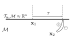
\includegraphics[width=0.5\textwidth]{figures/manifold.pdf}
    \caption{Manifold, tangent space, retraction and lift operations}
    \label{fig:manifold}
\end{figure}

As in \cite{sola2018micro}, we use the concept of composite manifold, which allows us to deal with a collection of elements $\bfx^i$ living in their respective manifold $\cM^i$, which very often occur in robotics. We define the composite manifold as the concatenation $\cM_c \triangleq \left<\cM^1, \dots, \cM^M \right>$. The element of this composite manifold is denoted by $\cX$.
We will also write a composite Lie group  equivalent of the retraction $\oplus$ and 
lift $\ominus$ operations. It consists in applying operations to individual elements of the manifold and its tangent space:

\begin{equation}
    \cX=
    \begin{bmatrix}
        \bfx^1 \\
        \vdots \\
        \bfx^M
    \end{bmatrix},
    \quad
    \cX \oplus \bftau
    =
    \begin{bmatrix}
        \bfx^1 \oplus \bftau^1 \\
        \vdots \\
        \bfx^M \oplus \bftau^M
    \end{bmatrix}
    \quad
    \cX_2 \ominus \cX_1
    =
    \begin{bmatrix}
        \bfx^1_2 \ominus \bfx^1_1 \\
        \vdots \\
        \bfx^M_2 \ominus \bfx^M_1
    \end{bmatrix}
    \label{eq:composite_retract}
\end{equation}



\subsection{Back to the MAP optimization problem}
\label{sec:manifold_GN}
Elements of the tangent space can be interpreted as steps that we can make to go from one point of the manifold to another.
This ties closely to the notion of Gaussian steps that we defined in \secRef{sec:gauss_newton_step}. We will now consider that the estimated state $\cX$
is an element of a composite manifold. In this case, the Gaussian steps of \eqRef{eq:gaussian_step}
are in the composite manifold tangent space and the step updates write:

\begin{equation}
    \check{\cX} := \check{\cX} \oplus \Delta \bfx^*
\end{equation}
%
obtained by solving
%
\begin{equation}
    \Delta \bfx^* = \argmin_{\Delta \bfx} ||\bfr(\check{\cX} \oplus \Delta \bfx)||^2.
\end{equation}


Concerning residual formulation in \eqRef{eq:error_expectation}, if the measurement $\bfz_i$ is itself an element of a manifold, 
then the vector subtraction needs to be replaced:

\begin{equation}
    \bfe_i(\cX_{S_i}) = \bfh(\cX_{S_i}) \ominus \bfz_i,
\end{equation}

Note that many state variables belong to vector spaces (such as the robot position), which are trivial manifolds. For those, the $\oplus$ and $\ominus$ operators
simply reduce to the addition and subtraction of Cartesian vectors.  



\subsection{Uncertainty on manifolds, Jacobians}
\label{sec:uncertainty_on_manifolds}
Our state variables are random variables approximated by multivariate Gaussian distribution, that can be summarized by their mean vector and covariance matrix.
These concepts need to be slightly modified to account for the manifold nature of some of these. We will see how to define Gaussian distribution on manifolds.
Let  $\bftau \in \Reals^n$ be a small perturbation around a point $\bar{\bfx} \in \cM$, so that we can write:
%
\begin{equation}
    \bfx = \bar{\bfx} \oplus \bftau, \quad \bftau = \bfx \ominus \bar{\bfx}
\end{equation}
%
where $\bar{\bfx}$ designates the mean value of the distribution on $\bfx$. 
We define a zero mean "Cartesian" Gaussian distribution on the tangent space, the covariance being defined as:

\begin{equation}
    \Cov_{\bfx} \triangleq \mathbb{E}[\bftau\bftau\tr] = \mathbb{E}[(\bfx \ominus \bar{\bfx})(\bfx \ominus \bar{\bfx})\tr] \in \Reals^{n \times n}
\end{equation}
%
where $\mathbb{E}[\cdot]$ denotes the expectation operator.
By a slight abuse of notation, we note that the manifold distribution is $\bfx \sim \Gaussian{\bfx}{\Cov_{\bfx}}$.

As an illustration, the group of unit quaternions $\mathbb{H} = \left\{ \bfq \in \Reals^4~|~\bfq \odot \bfq^*=1 \right\}$ under quaternion multiplication 
$\odot$ is a manifold (the $S^3$ sphere, p=4 and n=3) \cite{sola2012quaternion}. 
The tangent space is the set of antisymmetric matrices, which is isomorphic to the angle axis rotation vectors $\bftheta \in \Reals^3$.
If we naively define the covariance matrix of a quaternion as \mbox{$\mathbb{E}[(\bfq - \bar{\bfq})(\bfq - \bar{\bfq})\tr] \in \Reals^{4 \times 4}$}, 
this covariance matrix is ill-defined. The covariance must be more properly defined as a $3 \times 3$ real matrix on the angle axis space.

In general, covariances can be propagated through nonlinear function of random variables using the chain rule. For instance, if $\bfx \in \Reals^{n_x}$ and 
$\bfy \in \Reals^{n_y}$ are Cartesian multivariate Gaussian distribution related by the nonlinear function $f$, propagating the $\bfx$ covariance 
$\Cov_{\bfx} \in \Reals^{n_x \times n_x}$ through f writes:

\begin{equation}
    f~: \bfx \in \Reals^{n_x} \rightarrow \bfy \in \Reals^{n_y}, \quad \quad \Cov_{\bfy} \approx 
                \left.\frac{D f}{D \bfx} \right|_{\bfx}   \Cov_{\bfx}    \left.\frac{D \bfy}{D \bfx}\right|_{\bfx}\tr
    \label{eq:cov_propagation}
\end{equation}

The same equation applies for random variables $\bfx \in \cM_{\bfx}$ and $\bfy \in \cM_{\bfy}$ living on manifolds. The definition of Jacobians has however
to be redefined as:

\begin{equation}
    \frac{D f}{D \bfx} \triangleq \lim_{\bftau \to 0} \frac{f(\bfx \oplus \bftau) \ominus f(\bfx)}{\bftau}
\end{equation}

These Jacobians also play a central role in the derivation of the residual Jacobians \eqRef{eq:res_jacobian}.
Examples of manifold Jacobian derivations in the context of Lie groups can be found in \cite{sola2018micro}.  



\subsection{Lie groups for robotic state estimation}
\label{sec:lie_groups}
Riemannian geometry is enough to deal with optimization problems with variables living on smooth manifolds. However, many of these state variables, 
in the context of robotics, also exhibit a group structure, which gives them extra interesting properties.

A \textit{group} is an ordered pair ($\cG$, $\circ$) comprised of a set $\cG$ and a composition law $\circ$ that together satisfy the group axioms:

\begin{align}
    \text{Closure under}~\circ~:&~\bfx \circ \bfy \\ 
    \text{Associativity}~\circ~:&~(\bfx \circ \bfy) \circ \bfz = \bfx \circ (\bfy \circ \bfz) \\ 
    \text{Identity element}~\cE~:&~\bfx \circ \cE = \cE \circ \bfx = \bfx \\ 
    \text{Inverse existence}~\bfx^{-1}~:&~\bfx^{-1} \circ \bfx = \bfx \circ \bfx^{-1} = \cE
\end{align}
$\forall~\bfx,\bfy,\bfz \in \cG$.

Simply stated, a \text{Lie group} is a group whose elements live in a smooth manifold $\cM$.

A vector can represent a displacement from one point to another along a straight line in the euclidean space, or directly a point (displacement from the origin).
Analogously, an element of a Lie group represents either a path from one element to another along a geodesic of the manifold or directly an element of the group 
(displacement from the identity element $\cE$).

In particular, the identity element $\cE$ relates to a notion of a global reference from which each element of the manifold can be compared.
The tangent space at this element is called the Lie algebra $\mathfrak{m} \triangleq \cT_{\cE}\cM$.

Let us compute the retraction operations in the case of Lie groups. We will follow the example of 3D rotations as they are of great use in robotics and provide
good intuitions regarding the general behavior of Lie groups.
The group of 3D rotations is defined as the Special Orthogonal group in 3D: 
%
\begin{equation}
    \SO(3) = \left\{\Rot{}{} \in \text{GL}(n,\Reals) | \Rot{}{}\Rot{}{}\tr=\Rot{}{}\tr\Rot{}{}=\bfI,~det(\Rot{}{})=1\right\}
\end{equation}
%
under matrix multiplication.


Firstly, properties that make $SO(3)$ a group are immediate from the properties of matrix multiplication:
%
\begin{itemize}
    \item Closure under the matrix product
    \item Associativity through the matrix product
    \item Identity element $\bfI_3$
    \item Inverse element $\Rot{}{}^{-1} = \Rot{}{}\tr$ (from the group definition)
\end{itemize}

Let us explicit the manifold structure of $\SO(3)$.
It can be shown \cite{sola2018micro} that taking the time difference of a rotation matrices results in an element of its local tangent space:

\begin{equation}
    \dot{\Rot{}{}} = \Rot{}{} [\angvel{}{}]\hhat \in \cT_{\Rot{}{}}\SO(3)    
\end{equation}
%
where $[\cdot]\hhat$ is the skew-symmetric operator associated with the cross product. 
\mbox{$[\angvel{}{}]\hhat = \angvel{}{} \times \cdot$}. The Lie algebra $\so(3)$ is therefore the 3 dimensional vector space of antisymmetric matrices.
For a constant $\angvel{}{}$, this defines an ordinary differential equation (ODE) whose solution
is $\Rot{}{}(t)=\Rot{}{0}\exp([\angvel{}{}]\hhat t)$ where exp is the matrix exponential:

\begin{equation}
    \exp(\bfA) = \sum_{k=0}^{\infty} \frac{\bfA^k}{k!}.
\end{equation}

For $\SO(3)$ and most other Lie groups, properties of the Lie algebra simplify the infinite sum of the matrix exponential to a simpler closed-form formula. 
In the $\SO(3)$ case, this formula is known as the Rodrigues' formula:

\begin{equation}
    \Exp(\bftheta) = \exp([\bftheta]\hhat) = \bfI + [\bfu]\hhat\sin(\theta) + [\bfu]^{\wedge,2}(1 - \cos(\theta))
\end{equation}
%
where $\bftheta \triangleq \theta \bfu \in \Reals^3$ and $\theta$ is the norm of the rotation vector (angle in radians) and $\bfu$ its unitary direction.
Finally, we have denoted by $\Exp$ the composition of the $hat$ operator ($\bftheta\hhat \triangleq [\bftheta]\hhat \in \so(3)$) and the matrix exponential: $\Exp(\bftau) \triangleq \exp(\bftau\hhat)$. 
The inverse operation, that maps elements from the group to the Lie algebra, is defined as the $\Log$ map. A general representation of
Lie group operations can be found in \figRef{fig:lie_group}

With all of that in mind, the link with the Riemannian manifold terminology becomes clearer. We can compose a rotation with
an increment $\prescript{1}{}{\bftheta}$ taken in the tangent space at $\bfx_1$ to obtain another rotation: $\Rot{}{2} = \Rot{}{1}\Exp(\prescript{1}{}{\bftheta})$.
This corresponds to the $\oplus$ retraction operator. Conversely, the lift $\ominus$ corresponds to the application of The
logarithm on the relative rotation as described here:

\begin{align}
    \Rot{}{2} &= \Rot{}{1}\oplus \prescript{1}{}{\bftheta} = \Rot{}{1} \Exp(\prescript{1}{}{\bftheta})  \\ 
    \prescript{1}{}{\bftheta} &= \Rot{}{2}\ominus \Rot{}{1} = \Log(\Rot{}{1}\tr\Rot{}{2}) 
\end{align}

\begin{figure}[b]
    \centering
    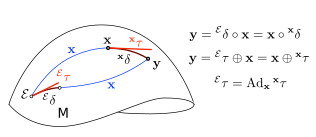
\includegraphics[width=0.7\textwidth]{figures/lie_group.pdf}
    \caption{Representations of a Lie group including the identity element $\cE$, operations of composition
    between increments and relations between a tangent space increment at the identity $\prescript{\cE}{}{\bftau}$ 
    and at the local element $\prescript{\bfx}{}{\bftau}$ through the adjoint matrix $\text{Ad}_{\bfx}$. Figure adapted from \cite{sola2018micro}.}
    \label{fig:lie_group} 
\end{figure}

\begin{figure}[h]
    \centering    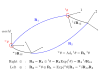
\includegraphics[width=0.7\textwidth]{figures/rotation_exp_log.pdf}
    \caption{Representation of $\SO(3)$ Lie groups operations. Note that we represented frames with different origins
    for better readability while the group elements only represent pure rotations (no translation). $world$ is the "global" reference 
    frame of the problem to which we assign the identity element of $\SO(3)$: $\bfI_3$. $1$ and $2$ are two frames of reference
    defined by their orientations \wrt $world$, $\Rot{}{1}$ and $\Rot{}{2}$. $\delta \Rot{}{12}$ is the relative rotation
    between elements $\Rot{}{1}$ and $\Rot{}{2}$ and can be computed using the exponential map on the angle axis $\bftheta$ expressed
    in $world$ or local frame, depending on whether we use the right or left $\oplus$ operator.}
    \label{fig:rotation_exp_log} 
\end{figure}

In robotics terms, $\prescript{1}{}{\bftheta}$ is the axis angle representation of the relative rotation $\prescript{1}{}{\delta \bfR}_{12} = \Rot{}{1}\tr\Rot{}{2}$ and
\textit{local} rotations represent the orientation of reference frames $\{1,2\}$ in a \textit{global} world reference frame. The identity element, therefore, corresponds 
to the world frame. 

Due to the general non-commutativity of the group operation, an additional $\oplus$ operator exists that retracts and composes vectors at the Lie algebra instead of
the local tangent space, the left-$\oplus$. The local operator, that corresponds to the manifold retraction, is called the right-$\oplus$. 
The Adjoint $\text{Ad}_{\bfx}\cM$ is an operator that maps elements from the local tangent space to the Lie algebra. 

\begin{equation}
    \prescript{\cE}{}{\bftau} = \text{Ad}_{\bfx}\cM \prescript{\bfx}{}{\bftau} 
\end{equation}

For rotation matrices, the adjoint matrix is $\text{Ad}_{\bfR}\SO(3)=\bfR$: to change the reference frame of the angle axis from local to global reference, it needs
to be rotated from one frame to another. Those operations are illustrated in \figRef{fig:rotation_exp_log}.


%
%
%
\section{Factor Graphs: a visual language for robotics estimation}
\label{sec:factor_graphs}

A crucial aspect of solving the MAP problem is the fact that the likelihood function is factorizable. This represents the fact that the problem
exhibits a particular structure that has important computational implications. We will first explain how this factorization can be described 
visually using a graphical model known as the \textit{Factor Graph} and then link this representation to the sparsity of the matrices involved
in solving the NLLS problem.


\subsection{Factor Graph representation}
Let us consider the toy example represented in \figRef{fig:toy_problem}. 
We wish to estimate the trajectory of a differential robot, that is its states at chosen timestamps called \textit{\keyframes}, and remarkable elements 
of the environment, called \textit{landmarks}. We suppose that this robot is equipped with an odometer, whose measurements integrated over time provide relative 
transformations between \keyframes, and an exteroceptive sensor that provides relative measurements between \keyframes~and landmarks.

\begin{figure}[h]
    \centering
    \begin{subfigure}{.49\linewidth}
        \centering
        \includegraphics[width=\textwidth]{figures/toy_example.pdf}
        \caption{\label{fig:toy_problem}}
    \end{subfigure}%
    \hfill
    \begin{subfigure}{.49\linewidth}
        \centering
        \includegraphics[width=\textwidth]{figures/toy_factor.pdf}
        \caption{\label{fig:toy_factor}}
    \end{subfigure}%
    \caption{(\subref{fig:toy_problem}): toy estimation problem, a differential drive robot equipped with an odometer moves in 
    an scene with landmarks represented by stars. (\subref{fig:toy_factor}): Factor Graph representation the problem, the estimated variables are represented by circles 
    (blue for robot \keyframes, green for landmarks) and factors by squares (orange for odometry, black for exteroceptive sensor, red for the prior).}
\end{figure}

In this case, the state variables are $\cX = \{ \bfx_1, \bfx_2, \bfx_3, l_1, l_2\}$  and measurements $\cZ = \{ z_{o,1}, z_{o,2}, z_{e,1}, z_{e,2}\}$.
We also apply a prior on the pose of the first \keyframe\ of the trajectory, which can be understood as fixing the frame origin of the reference 
frame in which the estimation is done.

The factorization of the likelihood of \eqRef{eq:likelihood_factorization} in this example writes:
%
\begin{align}
    p(\cX | \cZ) \propto 
    ~&{\color{Red} \phi_0({\color{Blue} \bfx_{0}})} \\ 
    ~&{\color{Orange} \phi_1({\color{Blue} \bfx_1}, {\color{Blue} \bfx_2}) \phi_2({\color{Blue} \bfx_2}, {\color{Blue} \bfx_3})} \\ 
    ~&{\color{Black} \phi_3({\color{Blue} \bfx_1}, {\color{Green} l_1}) \phi_4({\color{Blue} \bfx_2}, {\color{Green} l_1}, {\color{Green} l_2}) \phi_5({\color{Blue} \bfx_3}, {\color{Green} l_2})}
\end{align}

This factorization can be represented as a \textit{factor graph} as seen in \figRef{fig:toy_factor}. 
Factor graphs are popular probabilistic graphical models \cite{koller2009probabilistic} that can describe a vast family of statistical models \cite{loeliger2004introduction}.
In the general sense, a factor graph is a bipartite graph that represents the factorization of a function of several variables. In estimation , we use it to represent the factorized likelihood \eqRef{eq:factorized_likelihood}, or equivalently the NLLS problem \eqRef{eq:nlls_map_pbe}.

We adopt the visual notation commonly found in robotics: round nodes for variables, square nodes for factors, edges represent the dependency 
of each factor on a subset of variables. In the following parts, we will use the following terminology to designate factors depending on which variables they depend on:

\begin{itemize}
    \item \textbf{Unary factor} $\color{Red} \phi$: depends on a single \keyframes, obtained from a an absolute measurement (\eg a prior, GPS etc.)
    \item \textbf{Motion factor} $\color{Orange} \phi$: depends on successive \keyframes, obtained from a motion sensor (\eg wheel odometry, IMU etc.)
    \item \textbf{Relative} or \textbf{exteroceptive factor} $\phi$: depends on a \keyframe\ and a part of the map, a few landmarks in this case, obtained from exteroceptive sensors
\end{itemize}

Dellaert and Kaess \cite{dellaert2006square} were the first to
recognize the link between NLLS problems and factor graphs \cite{dong2019minisam}. Over the last two decades, they have grown in popularity among roboticists as a visual language to describe 
estimation problems \cite{dellaert2017factor} and planning problems \cite{dong2016motion}. As Frank Dellaert puts it \footnote{Citation from a recent talk,
see \href{https://www.youtube.com/watch?v=-yCC7mpgL4w}{this video}, around 15:30.}, factor graphs are "an amazing thing to write on blackboards".   
Aside from providing insights into the computational structure of the problems, they can be used as a common language between engineering teams
to convey insights about the nature of the problems to solve.

% The SLAM problem hereby represented as a factor graph in only one example of the vast family of estimation problems that can be modeled as a factor graph
% (other including \eg target tracking, structure-from-motion, control and planning \cite{}). 

The problems typically represented by factor graphs and found in estimation are very sparse.
Many specialized solvers \cite{grisetti2011g2o, kaess2012isam2, ila2017slam++} have been implemented to exploit this sparsity. 
Let us discuss the basis of sparse NLLS to conclude this chapter.
% A discussion of the particularities of factor-graph-based NNLS solvers can be found in \cite{dellaert2017factor, sola2017course}.




\subsection{Sparsity of the NLLS problem}

Each residual of the NLLS problem is a function of a small subset of the state variables. Therefore, each factor node in the Factor Graph representation of the problem is connected to but a few of the variable nodes. This makes for a graph with low connectivity. We will show that this low connectivity is linked to an important sparsity of the Jacobian matrix of the residuals.

The Jacobian matrix of the residuals $\bfJ \in \Reals^{M \times N}$ is a big sparse matrix of dimensions 
\begin{itemize}
    \item M rows = $\sum_{i=1}^{m}dim(\bfe_i) \rightarrow~$ the sum of residual dimensions
    \item N columns = $\sum_{i=1}^{n}dim(\cT_{\bfx_i}\cM_i)~\rightarrow$ the sum of variables tangent-spaces dimensions 
\end{itemize}   

Each block column corresponds to one of the state variables and each row corresponds to a residual. For each row, only the blocks corresponding to the
state variables that the residual depends on are non-zero. For instance, the matrix corresponding to the toy problem described in \figRef{fig:toy_problem} is:
\begin{equation}
    \bfJ=
    \begin{pmatrix}
        J^{0}_{\bfx_1} &   &     &     &     \\
       J^{o_1}_{\bfx_1} & J^{o_1}_{\bfx_2}  &     &     &     \\
                       & J^{o_2}_{\bfx_2}  & J^{o_2}_{\bfx_3}   &     &     \\
       J^{e_1}_{\bfx_1} &                  &     &  J^{o_2}_{\bfl_1}   &     \\
                       & J^{e_1}_{\bfx_2}  &     &  J^{e_1}_{\bfl_1}   &     \\
                       & J^{e_2}_{\bfx_2}  &     &     &  J^{e_2}_{\bfl_2}   \\
                       &                  & J^{e_3}_{\bfx_3}    &     &  J^{e_3}_{\bfl_2}   \\
    \end{pmatrix}
    \label{eq:sparse_jac}
\end{equation}



The approximate Hessian matrix $\bfH \in \Reals^{N \times N}$ displays a similarly remarkable sparsity that makes the resolution of the linear system
at each step very efficient. Algorithms such as the Schur complement \cite[A.5.5]{boyd2004convex}, Cholesky factorization \cite[C.3]{boyd2004convex}, 
and QR factorization \cite[C.5]{boyd2004convex} were applied by different authors to the problem of SLAM and estimation. 

\subsection{The algorithm (revisited)}
To tie things together, we now recapitulate the Gauss-Newton algorithm in the context of variables living on manifolds. 
We highlight the parts that differ from the regular Gauss-Newton algorithm with vector spaces.

\begin{enumerate}
    \item Initialize the state estimate at an initial value $\check{\cX} := \cX^0$ \\
    $\cX$ lives on a composite manifold. Its covariance is defined on the local tangent space of this manifold (see \secRef{sec:uncertainty_on_manifolds}).
    \item Approximate the NLLS cost function around the current estimate as a quadratic function \\
    The linear approximation is done using the notation of Jacobian on manifolds described in \secRef{sec:uncertainty_on_manifolds}.
    $\Delta \bfx$ is defined as the Cartesian representation of a composite tangent space element.  
    \item Find the optimal step $\Delta \bfx^*$ by solving a linear set of equations \eqRef{eq:linear_syst_GN} \\
    This part does not change. As mentioned in \secRef{sec:LM}, globalization of Gauss-Newton such as the Levenberg-Marquardt algorithm
    may alter the linear system to solved for increased performance.
    \item Update the current state estimate $\check{\cX} := \check{\cX} \oplus \Delta \bfx^*$ \\
    The update of the current state is done using the retraction operator $\oplus$ of the composite manifold \eqRef{eq:composite_retract}.
    \item Loop over steps 2-4 until convergence
\end{enumerate}

When the estimation algorithm has converged we can also obtain the covariance on the estimates (details and illustration are available in the 
appendix \chpRef{chp:MAP_covariance}). This is however a costly computation that is usually reserved for offline investigation of the estimation quality. 



\section{Conclusion}

We have described a general algorithm to solve NLLS problems with variables belonging to manifolds and weighted by covariance matrices. This problem
comes from framing the state estimation as a MAP problem and using multiple assumptions on the nature of the measurement models. These measurement models
are described as residuals weighted by their respective covariance matrices, representing the confidence we have in the sensor measurements. Factor Graphs can 
represent visually those problems and their connectivity is closely related to the sparsity of the linear problems appearing in the optimization algorithm.

In our opinion, two equally important research directions start from here: (i) finding new solvers extending these ideas to new sets of problems, such as multi-robot or multi-hypothesis problems, and (ii)
formulating new, efficient, and generalizable measurement models. This thesis mostly theoretically contributes to the direction of extending
the estimation model (ii) while we mostly rely on existing algorithms (i) to solve the subsequent problems.
A commonly used denomination in the context of robotics state estimation is to refer to the solver implementation as the \textit{backend} while the measurement models are referred to as \textit{front-ends}.

The next chapters each concentrate on a range of sensor modalities useful for legged robots:
object pose retrieval from vision algorithms, a generalized pre-integration theory for high rate sensors, legged robot kinematics, and the application 
of pre-integration to legged robots force measurements.





